\documentclass[10pt]{standalone}
\usepackage{amsmath}
\usepackage{amssymb}
\usepackage{pgf,tikz}
\usepackage{mathrsfs}
\usetikzlibrary{arrows,calc,positioning,shapes.symbols,shapes.geometric}
\pagestyle{empty}
\usepackage{siunitx}


\begin{document}
  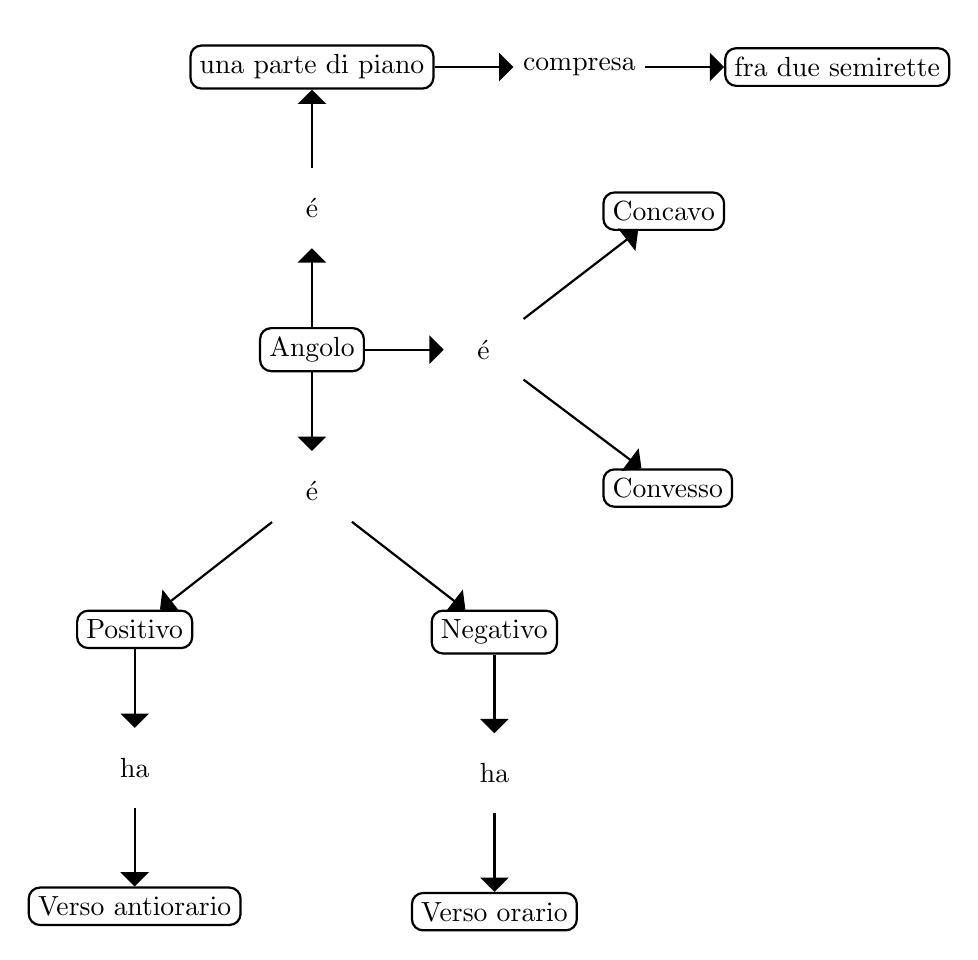
\begin{tikzpicture}
  \tikzset{every picture/.style={scale=0.3,every picture/.style={}}}
  \tikzset{main base/.style={draw,thick,text centered, }, }
  \tikzset{main node/.style={rectangle, draw,rounded corners,main base}, }
  %      
  %\tikzset{main verb/.style={minimum size=1cm}, }
  %\tikzset{linea/.style={-triangle 90}, }
  %\tikzset{main node2/.style={rectangle, draw,thick,
  %    text width=7em, text centered, rounded corners, minimum height=3em}, }
  \tikzset{main node2/.style={main node,
  		text width=7em, minimum height=3em}, }
  \tikzset{main verb/.style={minimum size=1cm}, }
  \tikzset{linea/.style={-triangle 90,thick,draw}}
  %\tikzset{linea/.style={-triangle 90,thick,draw}}
  \tikzset{linea2/.style={-triangle 90,draw}}
  \tikzset{primo/.style={circle,draw,inner sep=0pt,minimum size=1pt,thick}, }
    \node[main node] (1) {Angolo};
    \node[main verb] (2) [right =of 1]  {\'{e}};
  
   \node[main node] (3) [above right=of 2]  {Concavo};
   \node[main node] (4) [below right=of 2]  {Convesso};
   \node[main verb] (5) [below =of 1]  {\'{e}};
   \node[main node] (6) [below right=of 5]  {Negativo};
\node[main node] (7) [below left=of 5]  {Positivo};
    \node[main verb] (8) [below =of 6]  {ha};
\node[main node] (9) [below=of 8]  {Verso orario};
    \node[main verb] (10) [below =of 7]  {ha};
\node[main node] (11) [below=of 10]  {Verso antiorario};
\node[main verb] (12) [above =of 1]  {\'{e}};
\node[main node] (13) [above =of 12]  {una parte di piano};
\node[main verb] (14) [right =of 13]  {compresa};
\node[main node] (15) [right =of 14]  {fra due semirette};
\foreach \x /\y in{1/2,2/3,2/4,1/5,5/6,5/7,6/8,8/9,7/10,10/11,1/12,12/13,13/14,14/15}
  \path[linea] (\x) edge node {} (\y);
%  
\end{tikzpicture}
\end{document}